\documentclass[aspectratio=169]{beamer}
\setbeamertemplate{navigation symbols}{}
\usepackage{color, amsmath, comment, subfigure}
\usepackage{url}
\usepackage{ulem}

\usepackage{hyperref}
\hypersetup{
    colorlinks=true,
    linkcolor=blue,
    filecolor=magenta,      
    urlcolor=cyan,
}

%%%%%%%%%%%%%%%%%%%%%%%%%%
\title[]{Class slides for Tuesday, November 3:\\Disease models}
\author[]{Matthew J. Salganik}
\institute[]{}
\date[]{COS 597E/SOC 555 Limits to prediction\\Fall 2020, Princeton University}

\begin{document}
%%%%%%%%%%%%%%%%%%%%%%%%%%%
\frame{\titlepage}
%%%%%%%%%%%%%%%%%%%%%%%%%%%
\begin{frame}

\begin{center}
\LARGE{Vote}
\end{center}

\end{frame}
%%%%%%%%%%%%%%%%%%%%%%%%%%%%
\begin{frame}

\begin{center}
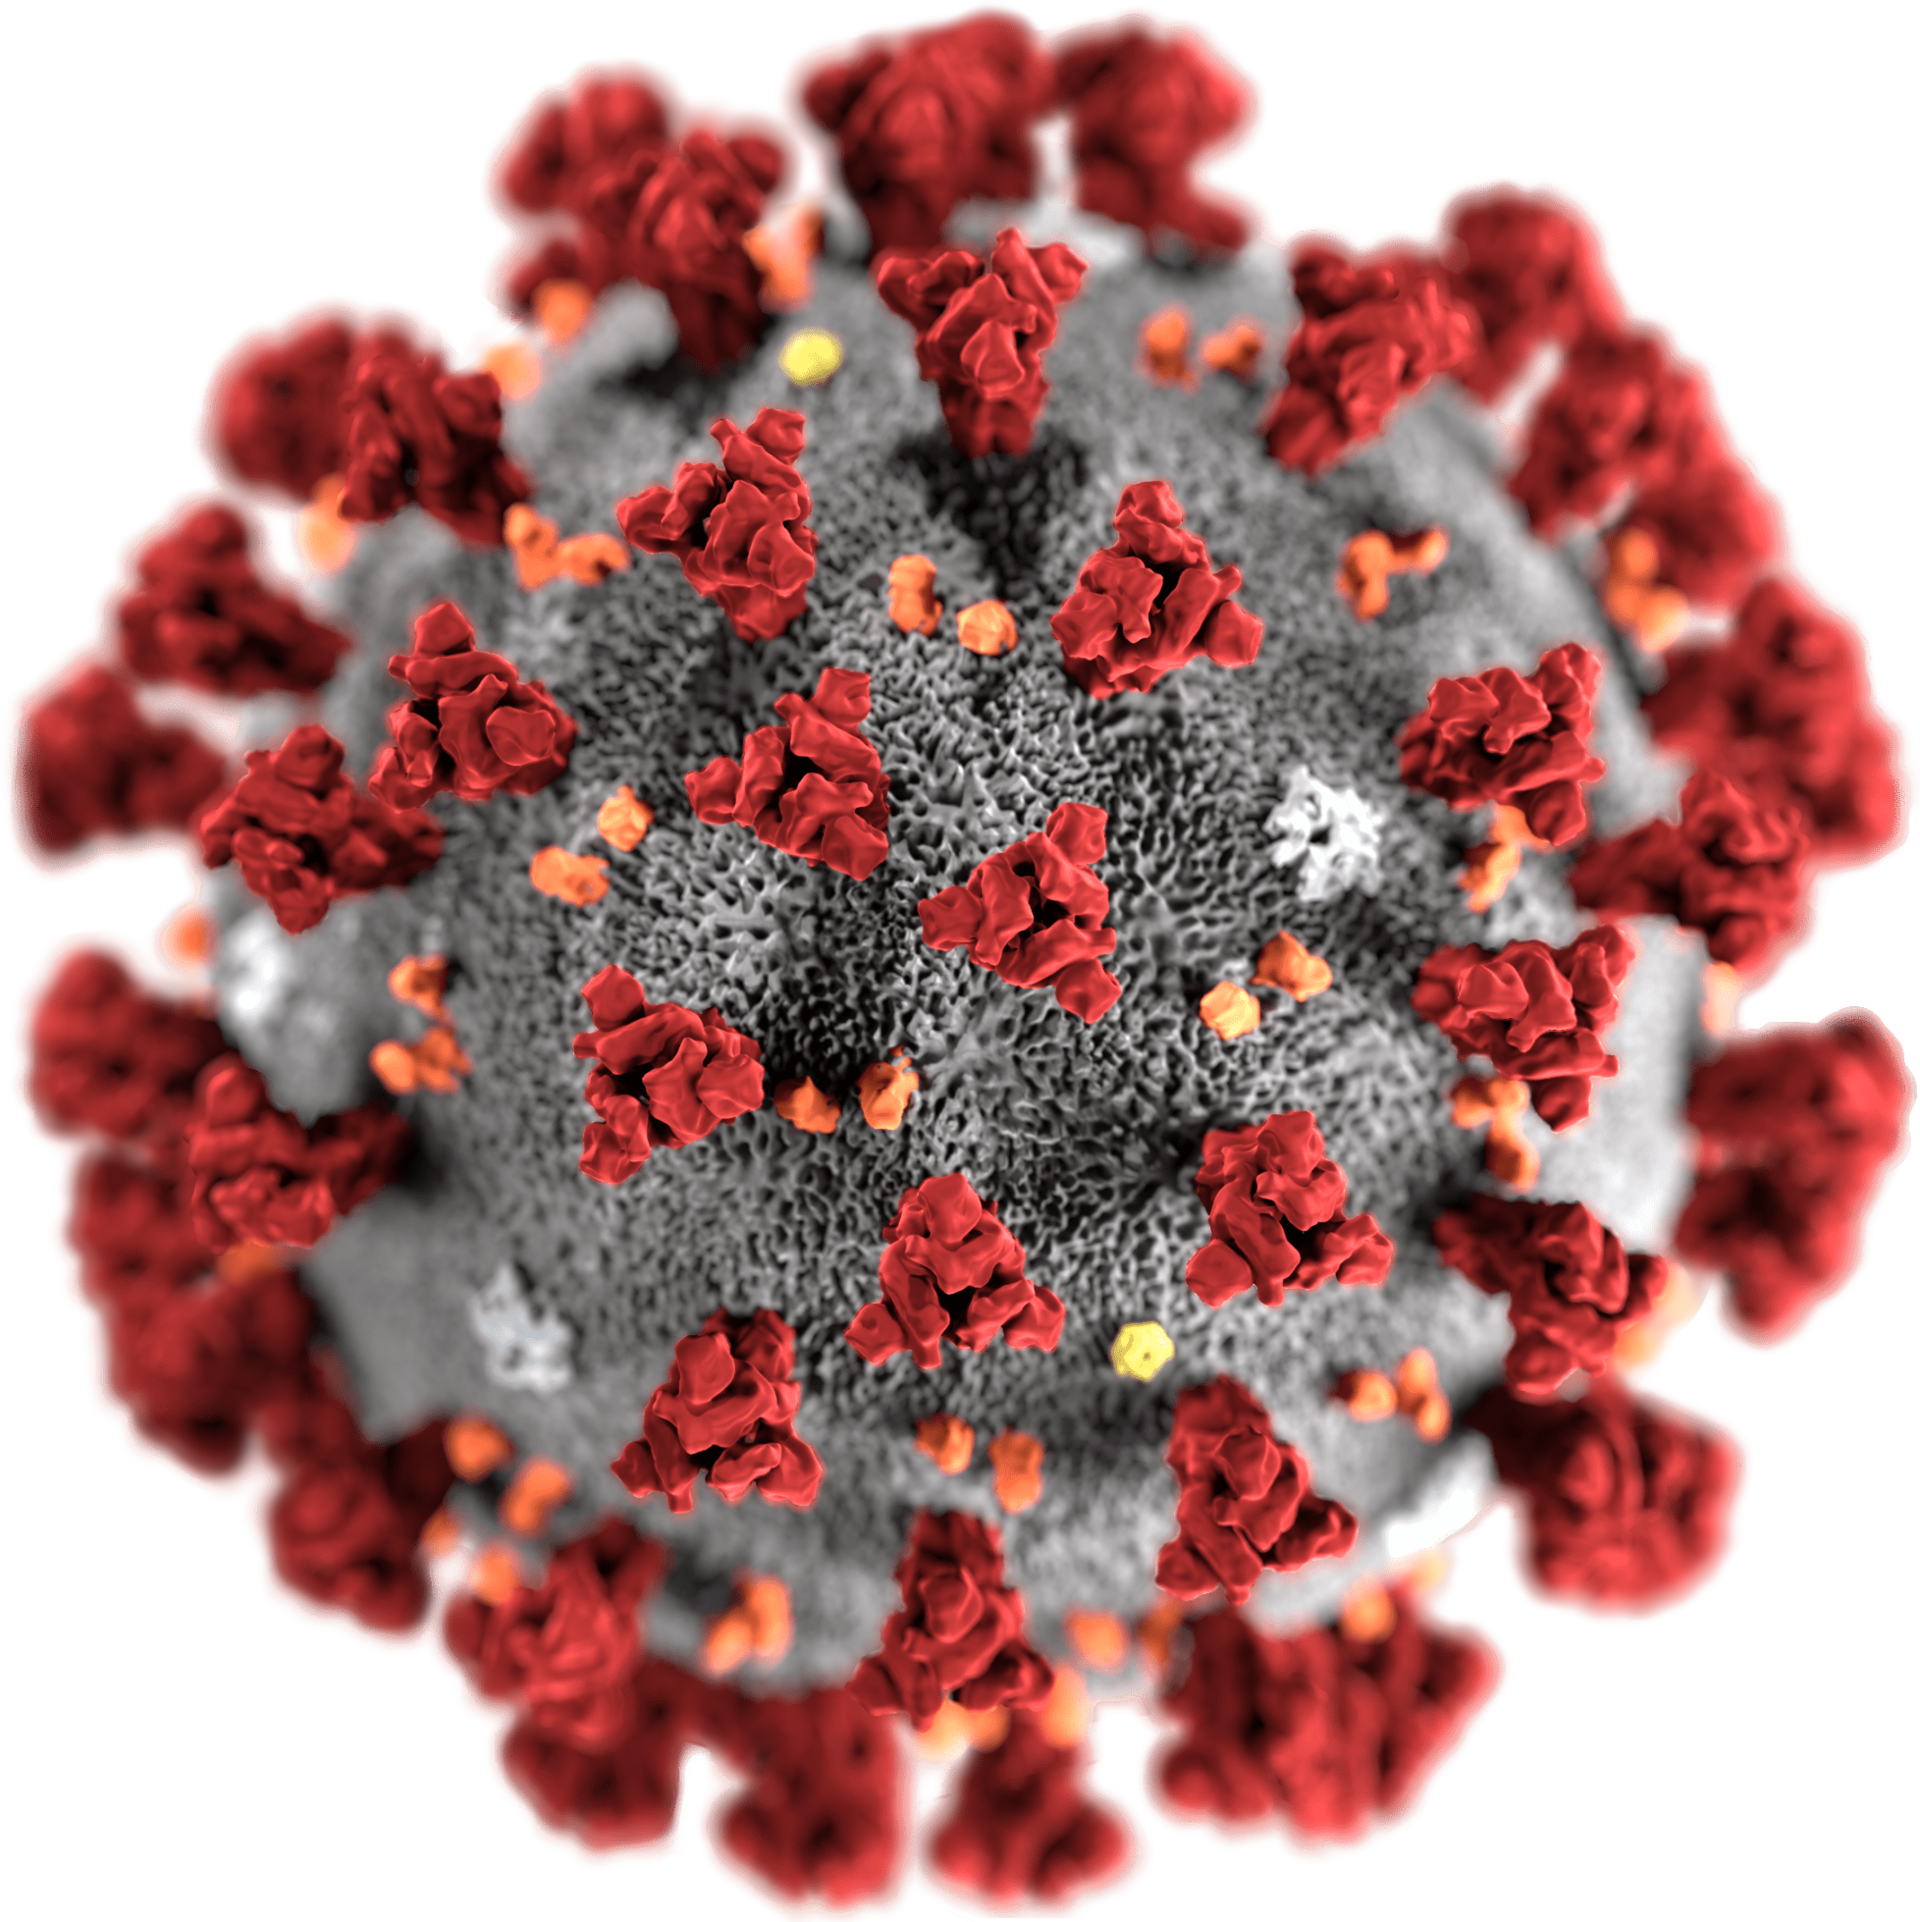
\includegraphics[height = 0.9\textheight]{figures/covid}
\end{center}

\vfill
\tiny{\url{https://phil.cdc.gov/Details.aspx?pid=23312}}
\end{frame}
%%%%%%%%%%%%%%%%%%%%%%%%%%%%
\begin{frame}

\begin{center}
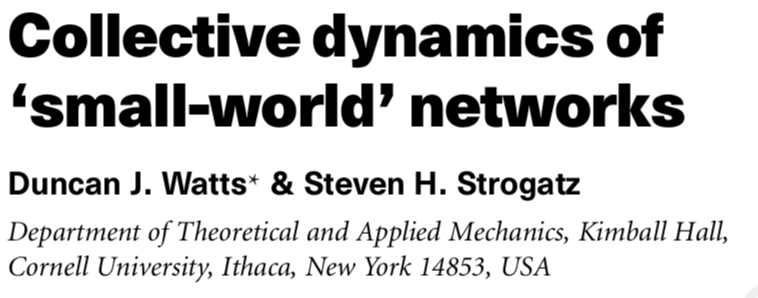
\includegraphics[width = 0.9\textwidth]{figures/watts_collective_1998_title}
\end{center}

\end{frame}
%%%%%%%%%%%%%%%%%%%%%%%%%%%%
\begin{frame}

\begin{center}
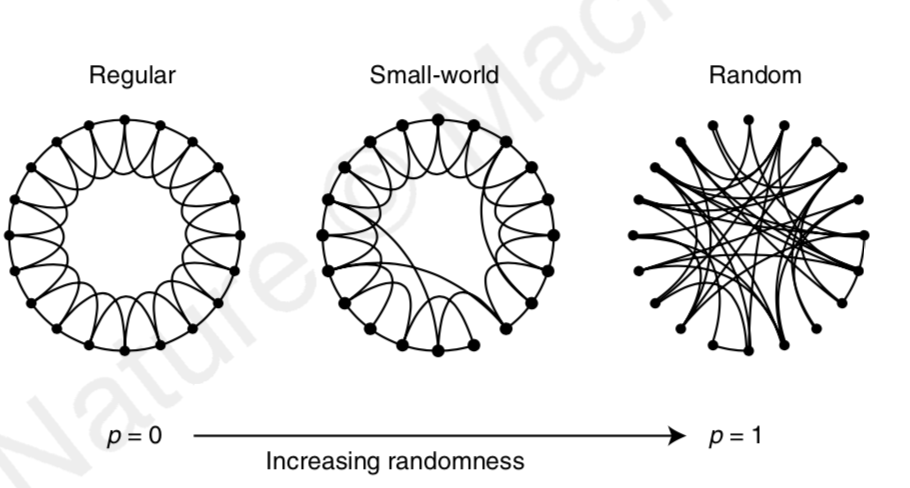
\includegraphics[width = 0.9\textwidth]{figures/watts_collective_1998_fig1}
\end{center}

\end{frame}
%%%%%%%%%%%%%%%%%%%%%%%%%%%%
\begin{frame}

\begin{center}
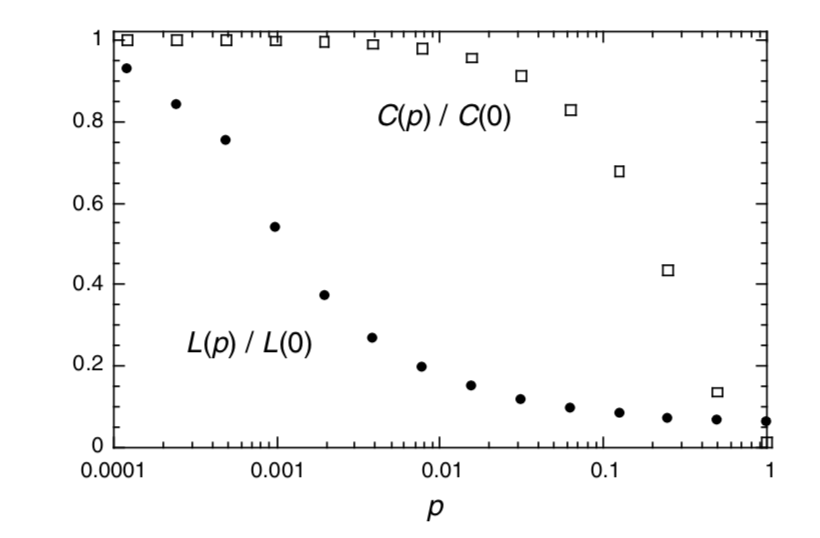
\includegraphics[width = 0.9\textwidth]{figures/watts_collective_1998_fig2}
\end{center}

\end{frame}
%%%%%%%%%%%%%%%%%%%%%%%%%%%%%
\begin{frame}

\begin{center}
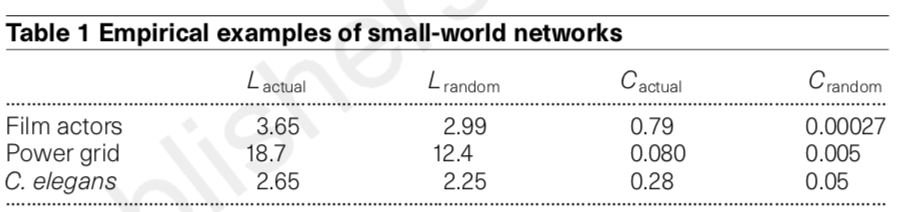
\includegraphics[width = 0.9\textwidth]{figures/watts_collective_1998_tab1}
\end{center}

\end{frame}
%%%%%%%%%%%%%%%%%%%%%%%%%%%%%
\begin{frame}

\begin{columns}[c]
  \column{.5\textwidth}
  \begin{center}
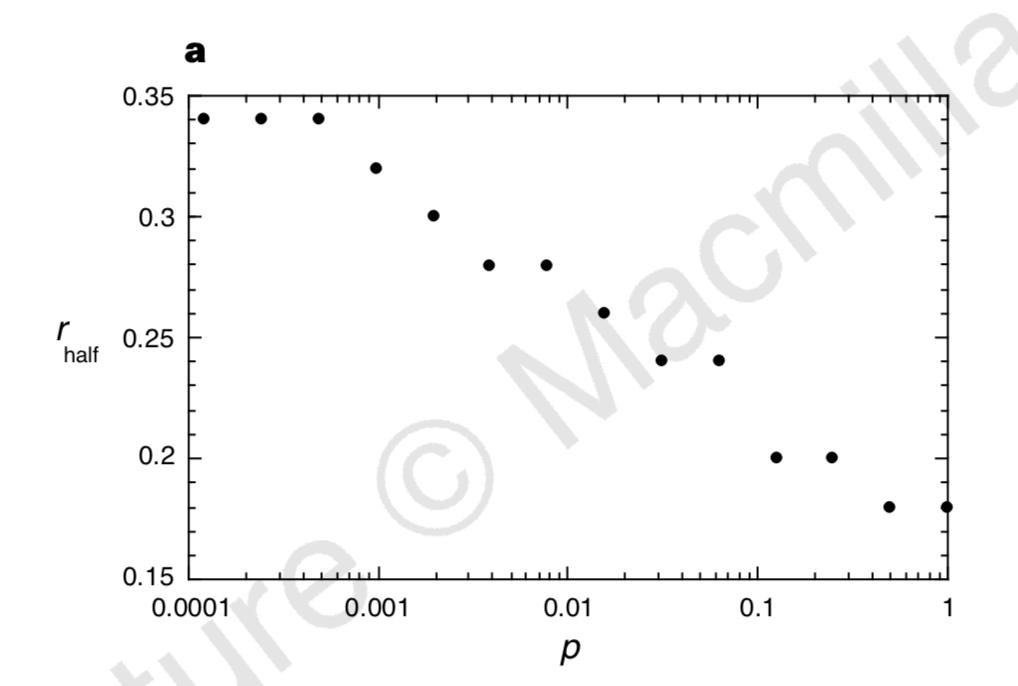
\includegraphics[width = 0.9\textwidth]{figures/watts_collective_1998_fig3a}
  \end{center}
   \column{.5\textwidth} 
   \begin{center}
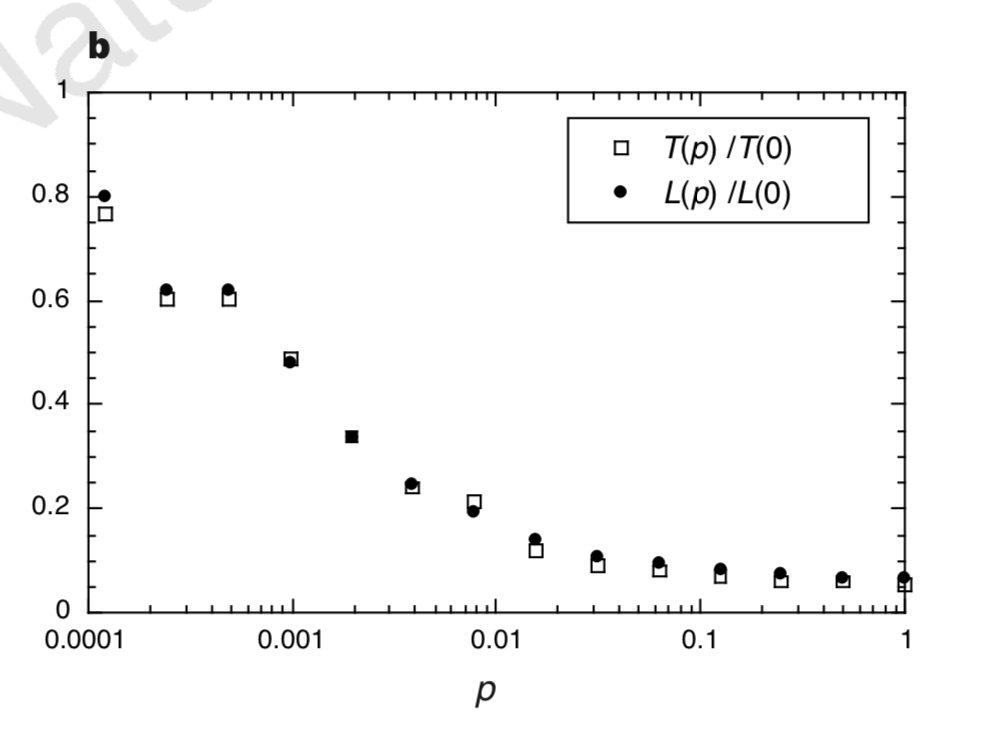
\includegraphics[width = 0.9\textwidth]{figures/watts_collective_1998_fig3b}
  \end{center}
\end{columns}

\vfill
Main result: Small change in network structure can make big difference for how infectious a disease needs to be to spread (a) and how quickly a highly infectious disease spreads (b)

\end{frame}
%%%%%%%%%%%%%%%%%%%%%%%%%%%%%
\begin{frame}

Main take away for our class
\begin{itemize}
\item sometimes small changes in network structure can make a big difference in disease spread, but sometimes large changes can make no difference
\end{itemize}

\end{frame}
%%%%%%%%%%%%%%%%%%%%%%%%%%%%%
\begin{frame}

\begin{center}
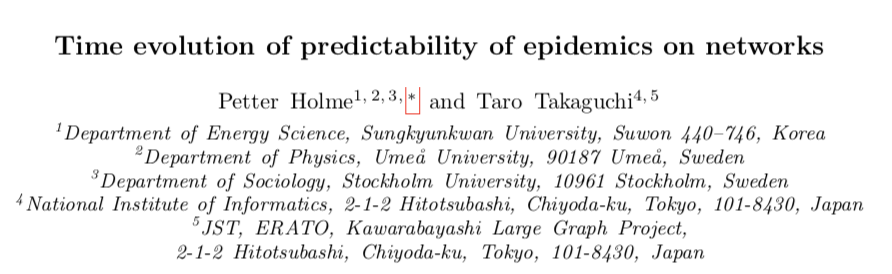
\includegraphics[width = 0.9\textwidth]{figures/holme_time_2015_title}
\end{center}

\end{frame}
%%%%%%%%%%%%%%%%%%%%%%%%%%%%%
\begin{frame}

\begin{itemize}
\item SIR model on different networks
\pause
\item $\beta$ probability of one person infecting another, $\nu$ rate of recovery (from I to R)
\pause
\item Assume that we have perfect information about the network and disease state of each person (they call this ``limit of maximum information'') 
\end{itemize}

\end{frame}
%%%%%%%%%%%%%%%%%%%%%%%%%%%%%
\begin{frame}

\begin{center}
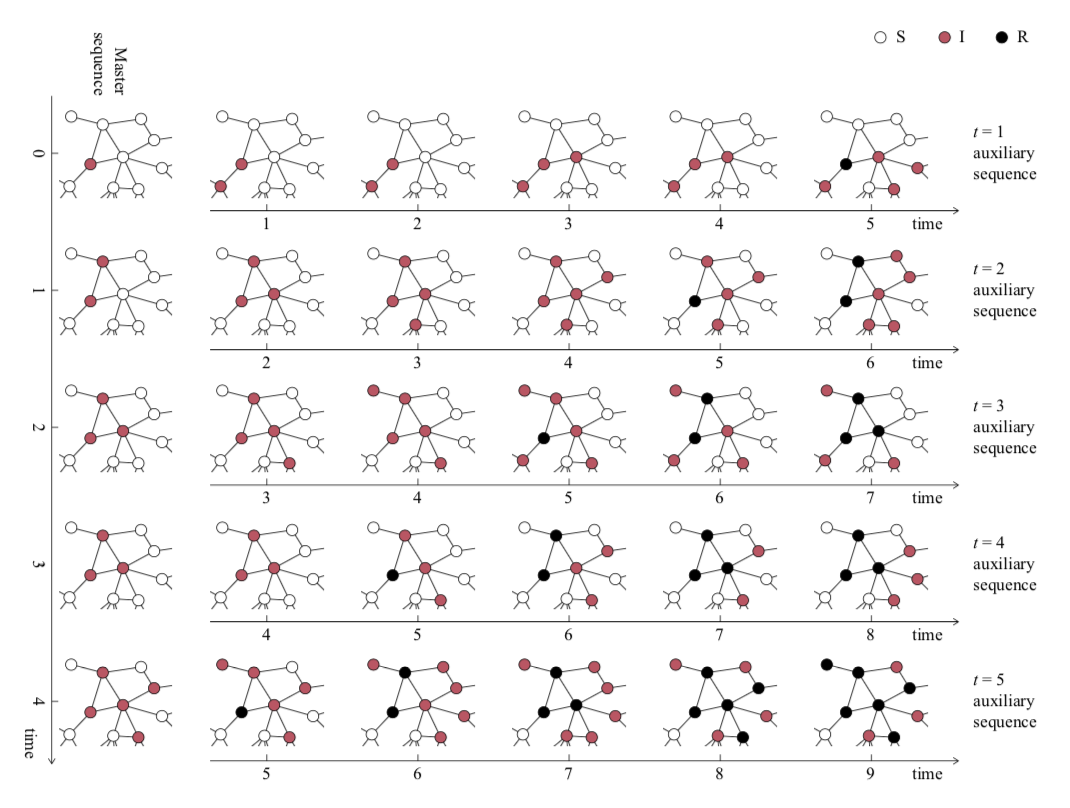
\includegraphics[height = 0.9\textheight]{figures/holme_time_2015_fig1}
\end{center}

\end{frame}
%%%%%%%%%%%%%%%%%%%%%%%%%%%%%
\begin{frame}

\begin{center}
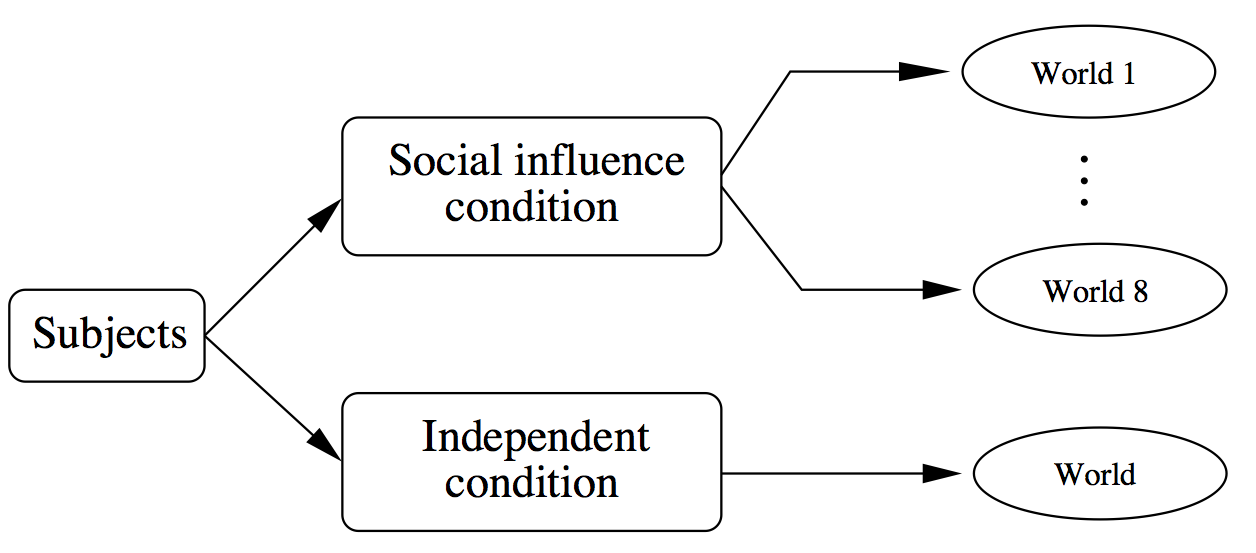
\includegraphics[width = 0.9\textwidth]{figures/musiclab_exp_design}
\end{center}

\end{frame}
%%%%%%%%%%%%%%%%%%%%%%%%%%%%%%
\begin{frame}

\begin{center}
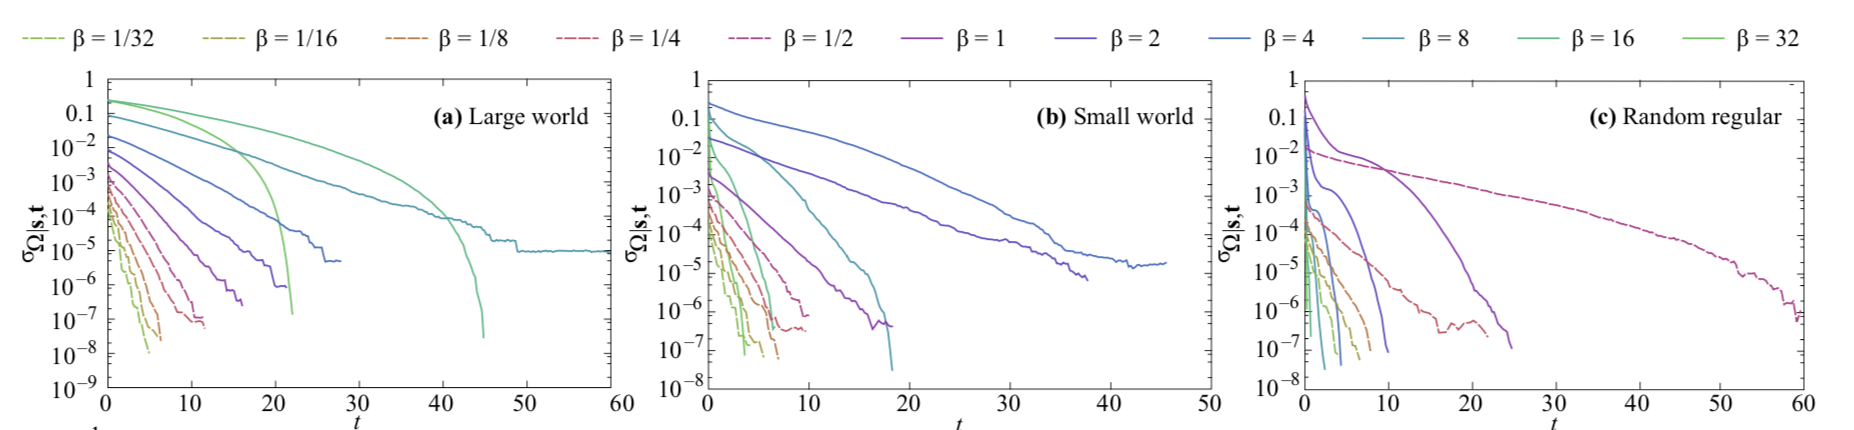
\includegraphics[width = 0.9\textwidth]{figures/holme_time_2015_fig3_toprow}
\end{center}

\vfill
Main result: Unpredictability of outbreak size $(\Omega)$ goes down exponentially fast
\end{frame}
%%%%%%%%%%%%%%%%%%%%%%%%%%%%%
\begin{frame}

\begin{center}
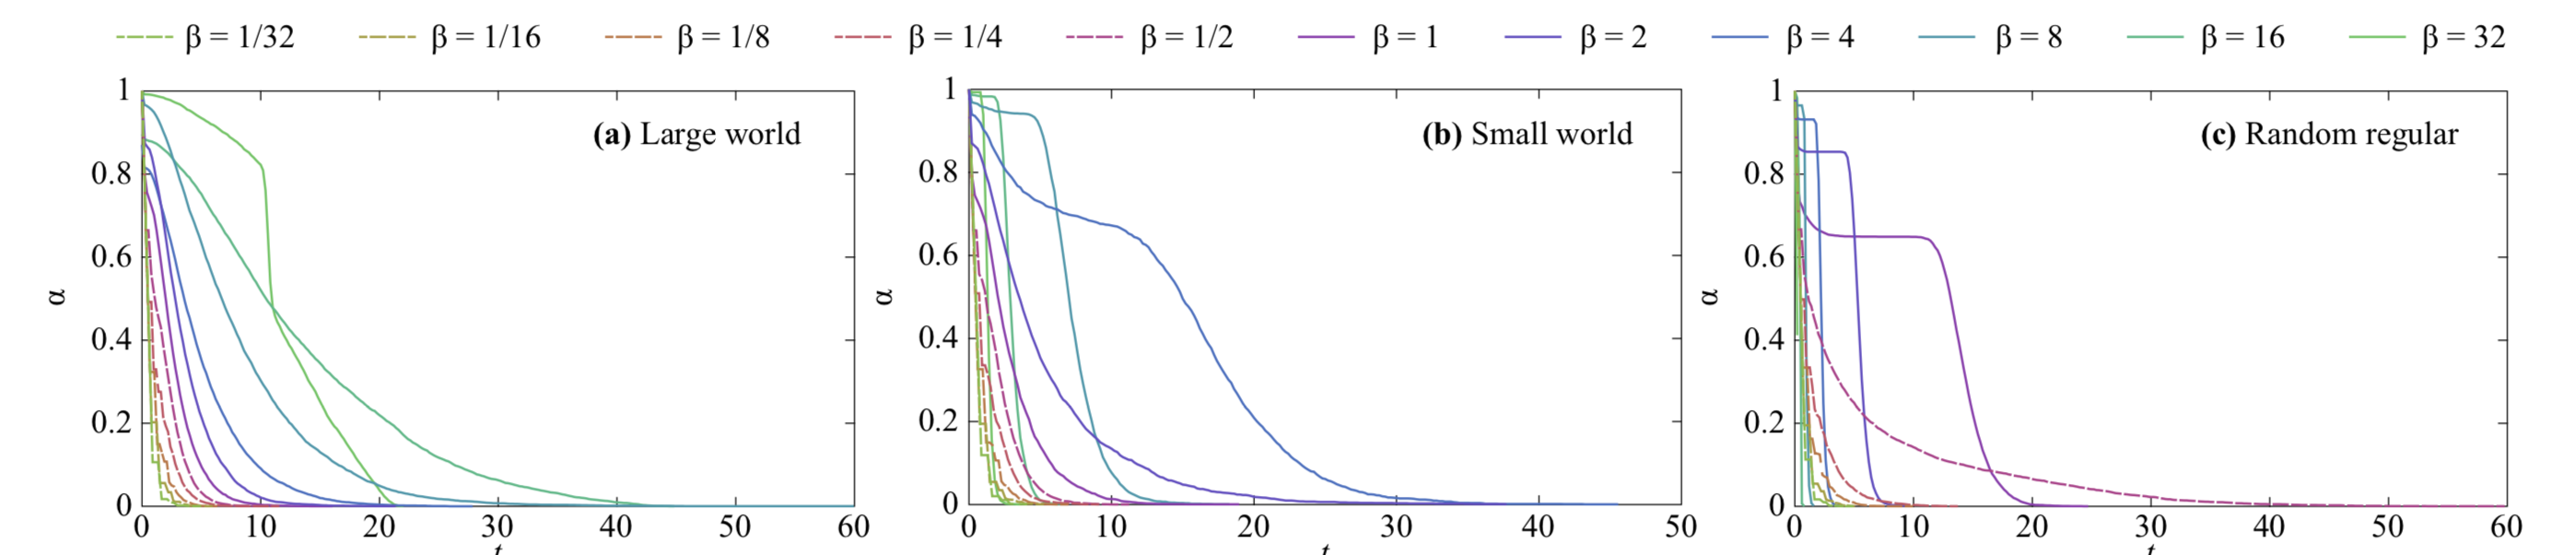
\includegraphics[width = 0.9\textwidth]{figures/holme_time_2015_fig4_toprow}
\end{center}

\vfill
Main result: Fraction of surviving outbreaks decreases over time. For large world, most infectious survive the longest, for small world and regular random, intermediate infectiousness survives the longest.
\end{frame}
%%%%%%%%%%%%%%%%%%%%%%%%%%%%%
\begin{frame}

\begin{center}
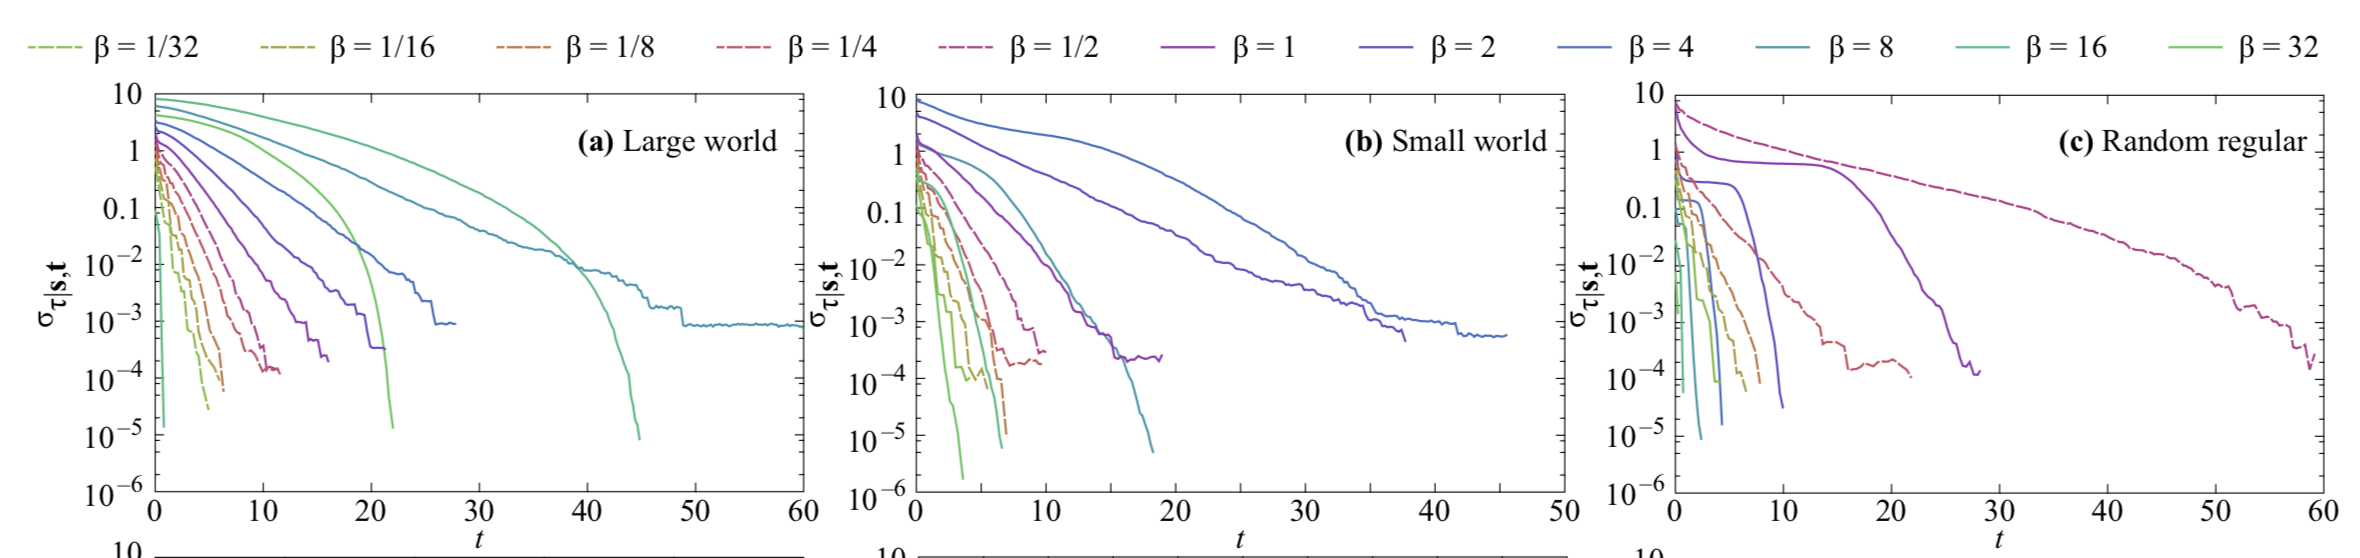
\includegraphics[width = 0.9\textwidth]{figures/holme_time_2015_fig7_toprow}
\end{center}

\vfill
Main result: Unpredictability of extinction time $(\tau)$ goes down exponentially fast
\end{frame}
%%%%%%%%%%%%%%%%%%%%%%%%%%%%%
\begin{frame}

2 main take aways
\begin{itemize}
\item using simulation it is possible to study how unpredictability changes over time
\pause
\item outbreaks are most unpredictability right at the beginning and get much easier to predict over time in this toy setting. Think back to ex-ante vs peeking strategies. think forward to prediction vs surveillance. 
\end{itemize}

\end{frame}
%%%%%%%%%%%%%%%%%%%%%%%%%%%%%
\begin{frame}

\begin{center}
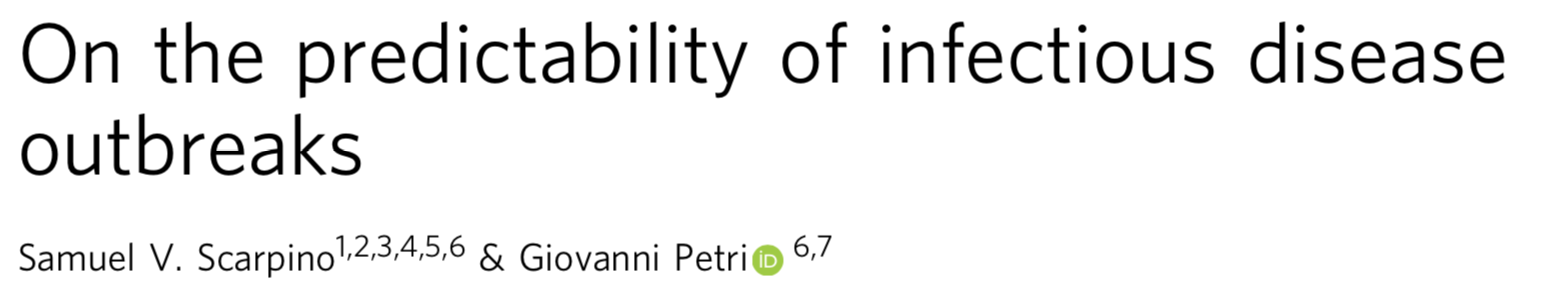
\includegraphics[width = 0.9\textwidth]{figures/scarpino_on_2019_title}
\end{center}

\end{frame}
%%%%%%%%%%%%%%%%%%%%%%%%%%%%%%
\begin{frame}

\url{https://www.youtube.com/watch?v=LaTAq1NUTPE}

\end{frame}
%%%%%%%%%%%%%%%%%%%%%%%%%%%%%%
\begin{frame}

\begin{center}
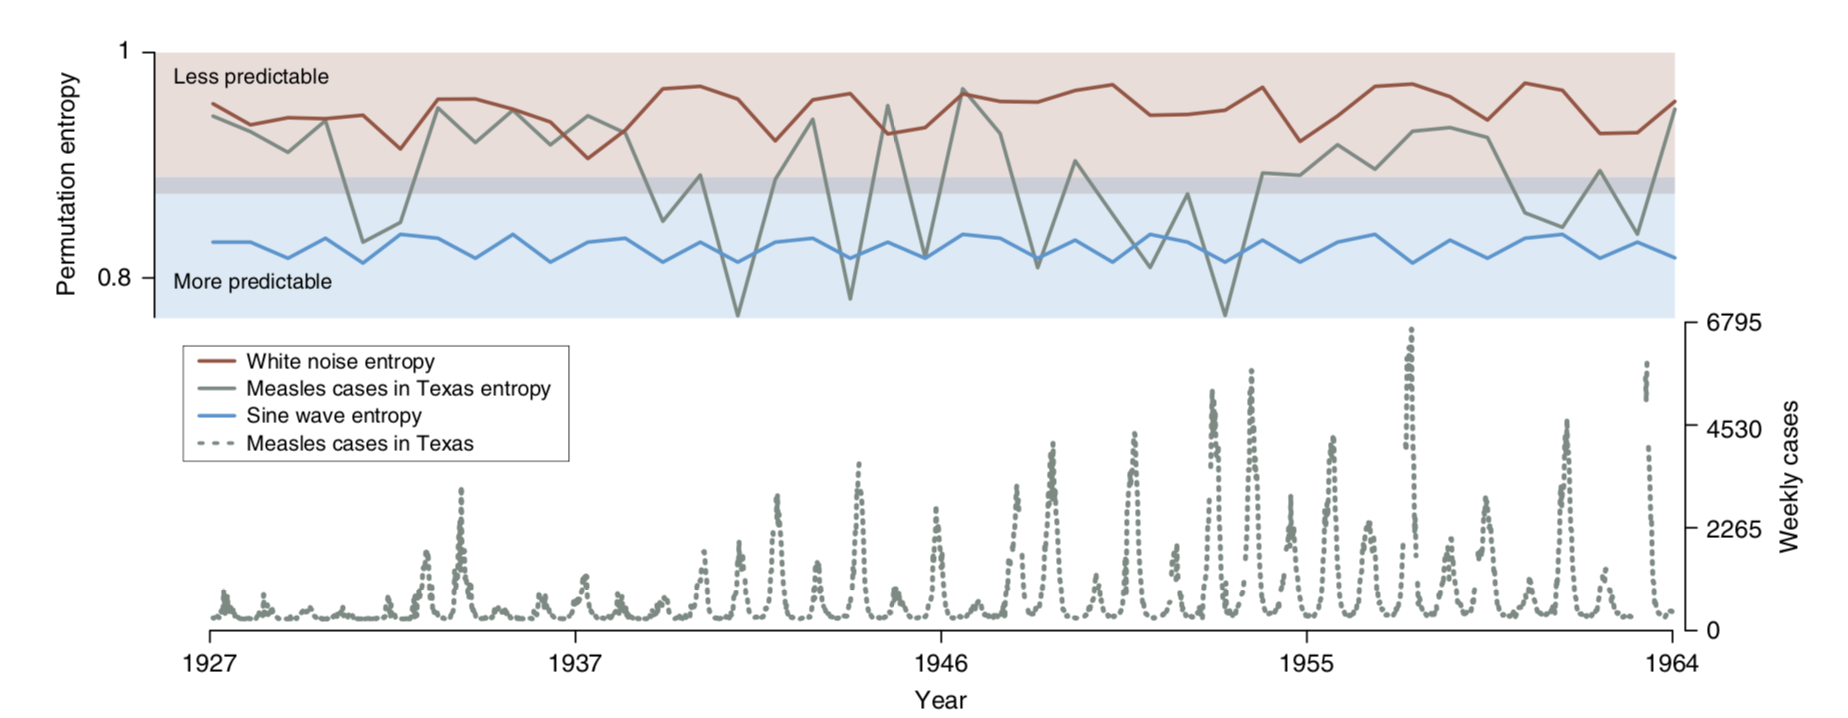
\includegraphics[width = 0.9\textwidth]{figures/scarpino_on_2019_fig1}
\end{center}

\vfill
Is being correlated with forecast limits in other systems enough?
\end{frame}
%%%%%%%%%%%%%%%%%%%%%%%%%%%%%%
\begin{frame}

\begin{center}
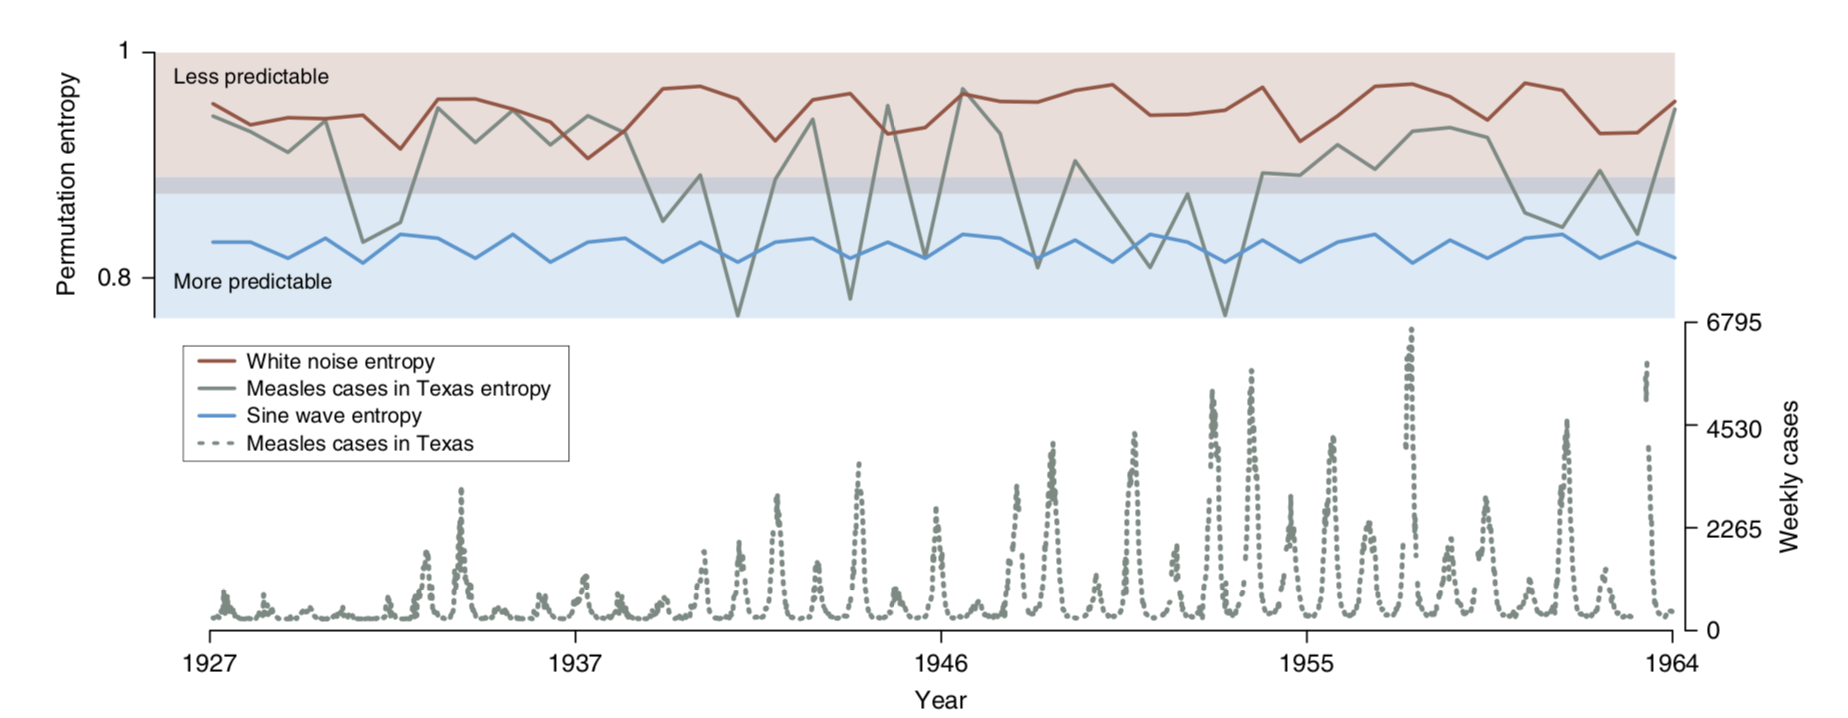
\includegraphics[width = 0.9\textwidth]{figures/scarpino_on_2019_fig1}
\end{center}

\vfill
For the sake of this class, we will assume that these results are robust with respect to how one calculates permutation entropy
\end{frame}
%%%%%%%%%%%%%%%%%%%%%%%%%%%%%%
\begin{frame}

\begin{center}
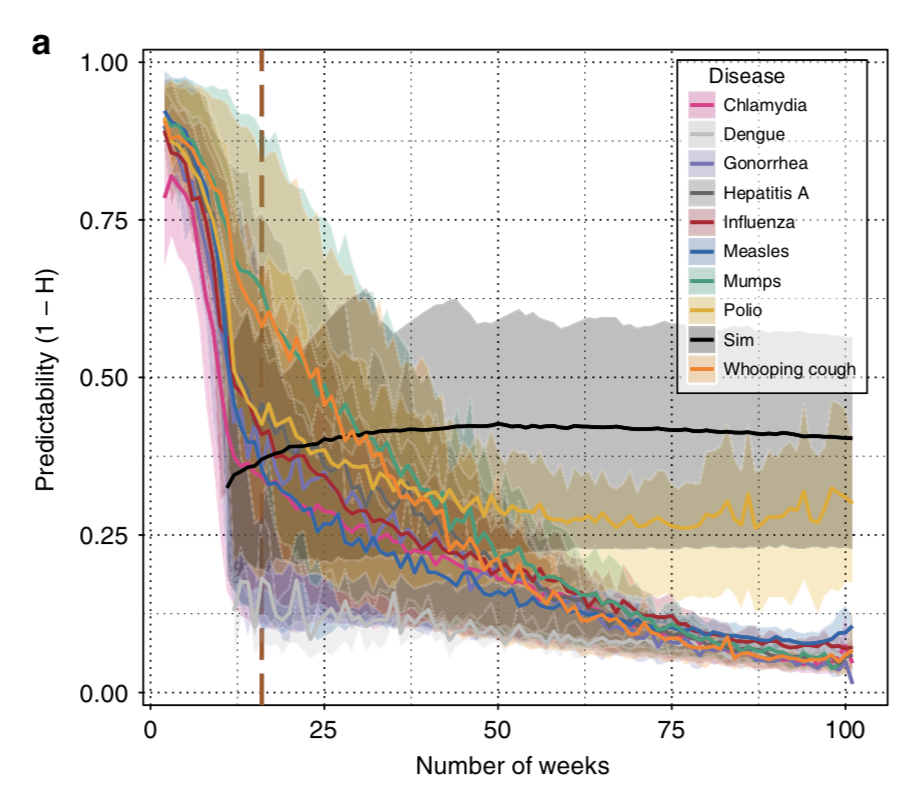
\includegraphics[width = 0.5\textwidth]{figures/scarpino_on_2019_fig2a}
\end{center}

\begin{center}
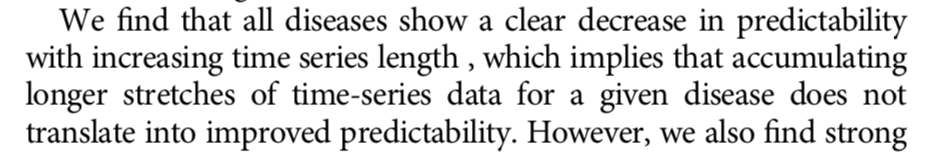
\includegraphics[width = 0.9\textwidth]{figures/scarpino_on_2019_more_data_less_predictability}
\end{center}

\end{frame}
%%%%%%%%%%%%%%%%%%%%%%%%%%%%%%
\begin{frame}

\begin{center}
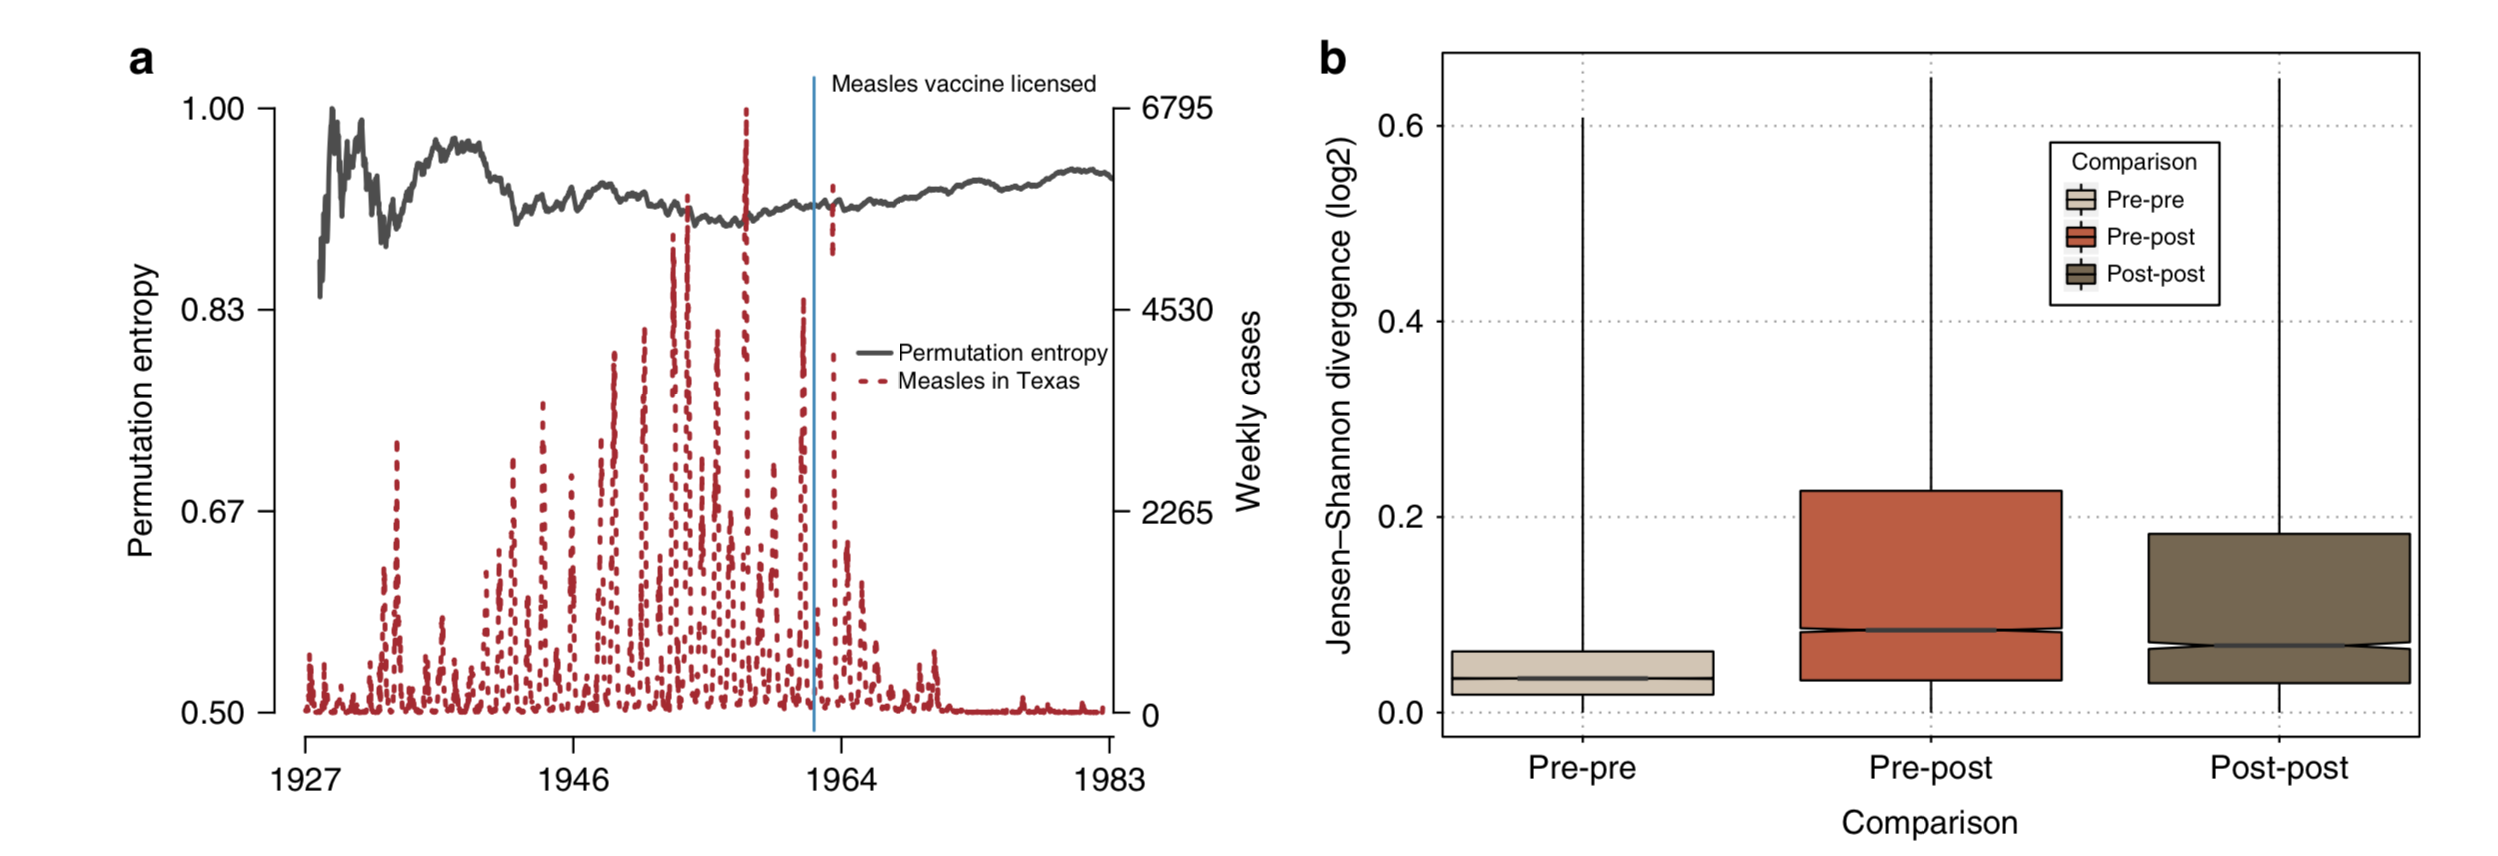
\includegraphics[width = 0.9\textwidth]{figures/scarpino_on_2019_fig4}
\end{center}

\begin{center}
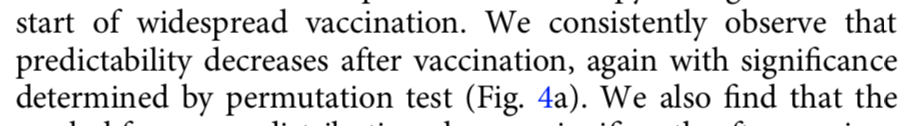
\includegraphics[width = 0.9\textwidth]{figures/scarpino_on_2019_predictability_after_vaccination}
\end{center}

\pause
\vfill What information would you need to predict what will happen after a vaccine is introduced?
\end{frame}
%%%%%%%%%%%%%%%%%%%%%%%%%%%%%%
\begin{frame}

\begin{center}
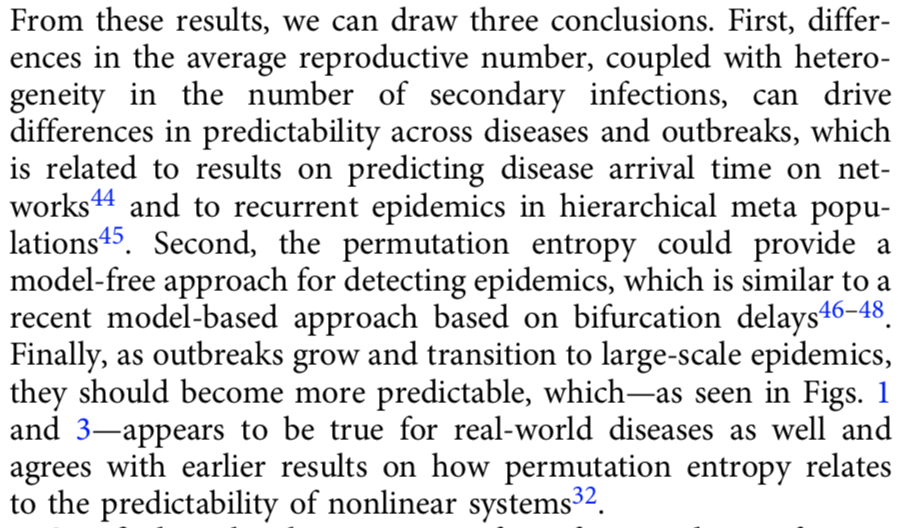
\includegraphics[width = 0.9\textwidth]{figures/scarpino_on_2019_conclusions}
\end{center}

\end{frame}
%%%%%%%%%%%%%%%%%%%%%%%%%%%%%%
\begin{frame}

\begin{center}
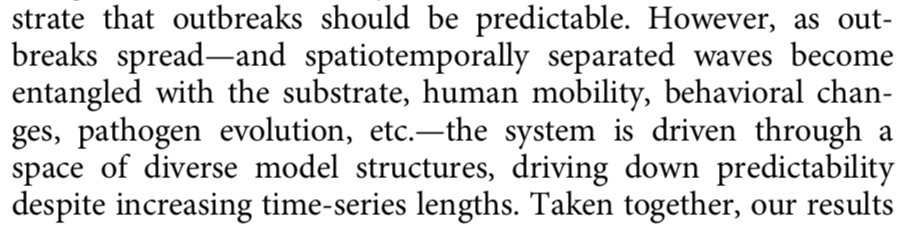
\includegraphics[width = 0.9\textwidth]{figures/scarpino_on_2019_stuff_changes}
\end{center}

\end{frame}
%%%%%%%%%%%%%%%%%%%%%%%%%%%%%%
\begin{frame}

Stepping back
\begin{itemize}
\item We can make precise statements about toy models (Holme and Takaguchi) or imprecise statements about real data (Scarpino and Petri). Ugh.
\pause
\item All these papers assume an isolated system.
\end{itemize}

\end{frame}
%%%%%%%%%%%%%%%%%%%%%%%%%%%%%%%%%%%%%%%
\begin{frame}

\begin{center}
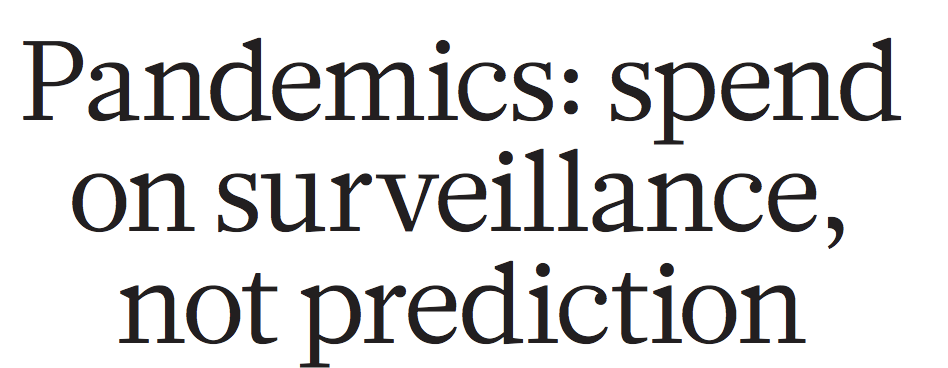
\includegraphics[width = 0.9\textwidth]{figures/holmes_pandemics_2018_title}
\end{center}

\vfill
Measuring the present is more important than predicting the future, and it requires that we change our focus.

\end{frame}
%%%%%%%%%%%%%%%%%%%%%%%%%%%%%%%%%%%%%%%%
\begin{frame}

My 3 takeaways:
\begin{itemize}
\item Sometimes small changes can make a big difference, and sometimes big changes can make a small difference
\pause
\item It is hard to learn about predictability in realistic systems
\pause
\item Prediction might be less important than measurement
\end{itemize}

\end{frame}
%%%%%%%%%%%%%%%%%%%%%%%%%%
\frame{\titlepage}


\end{document}
